\providecommand{\main}{../../../..}
\documentclass[\main/dresen_thesis.tex]{subfiles}

\begin{document}
  \begin{figure}[tb]
    \centering
    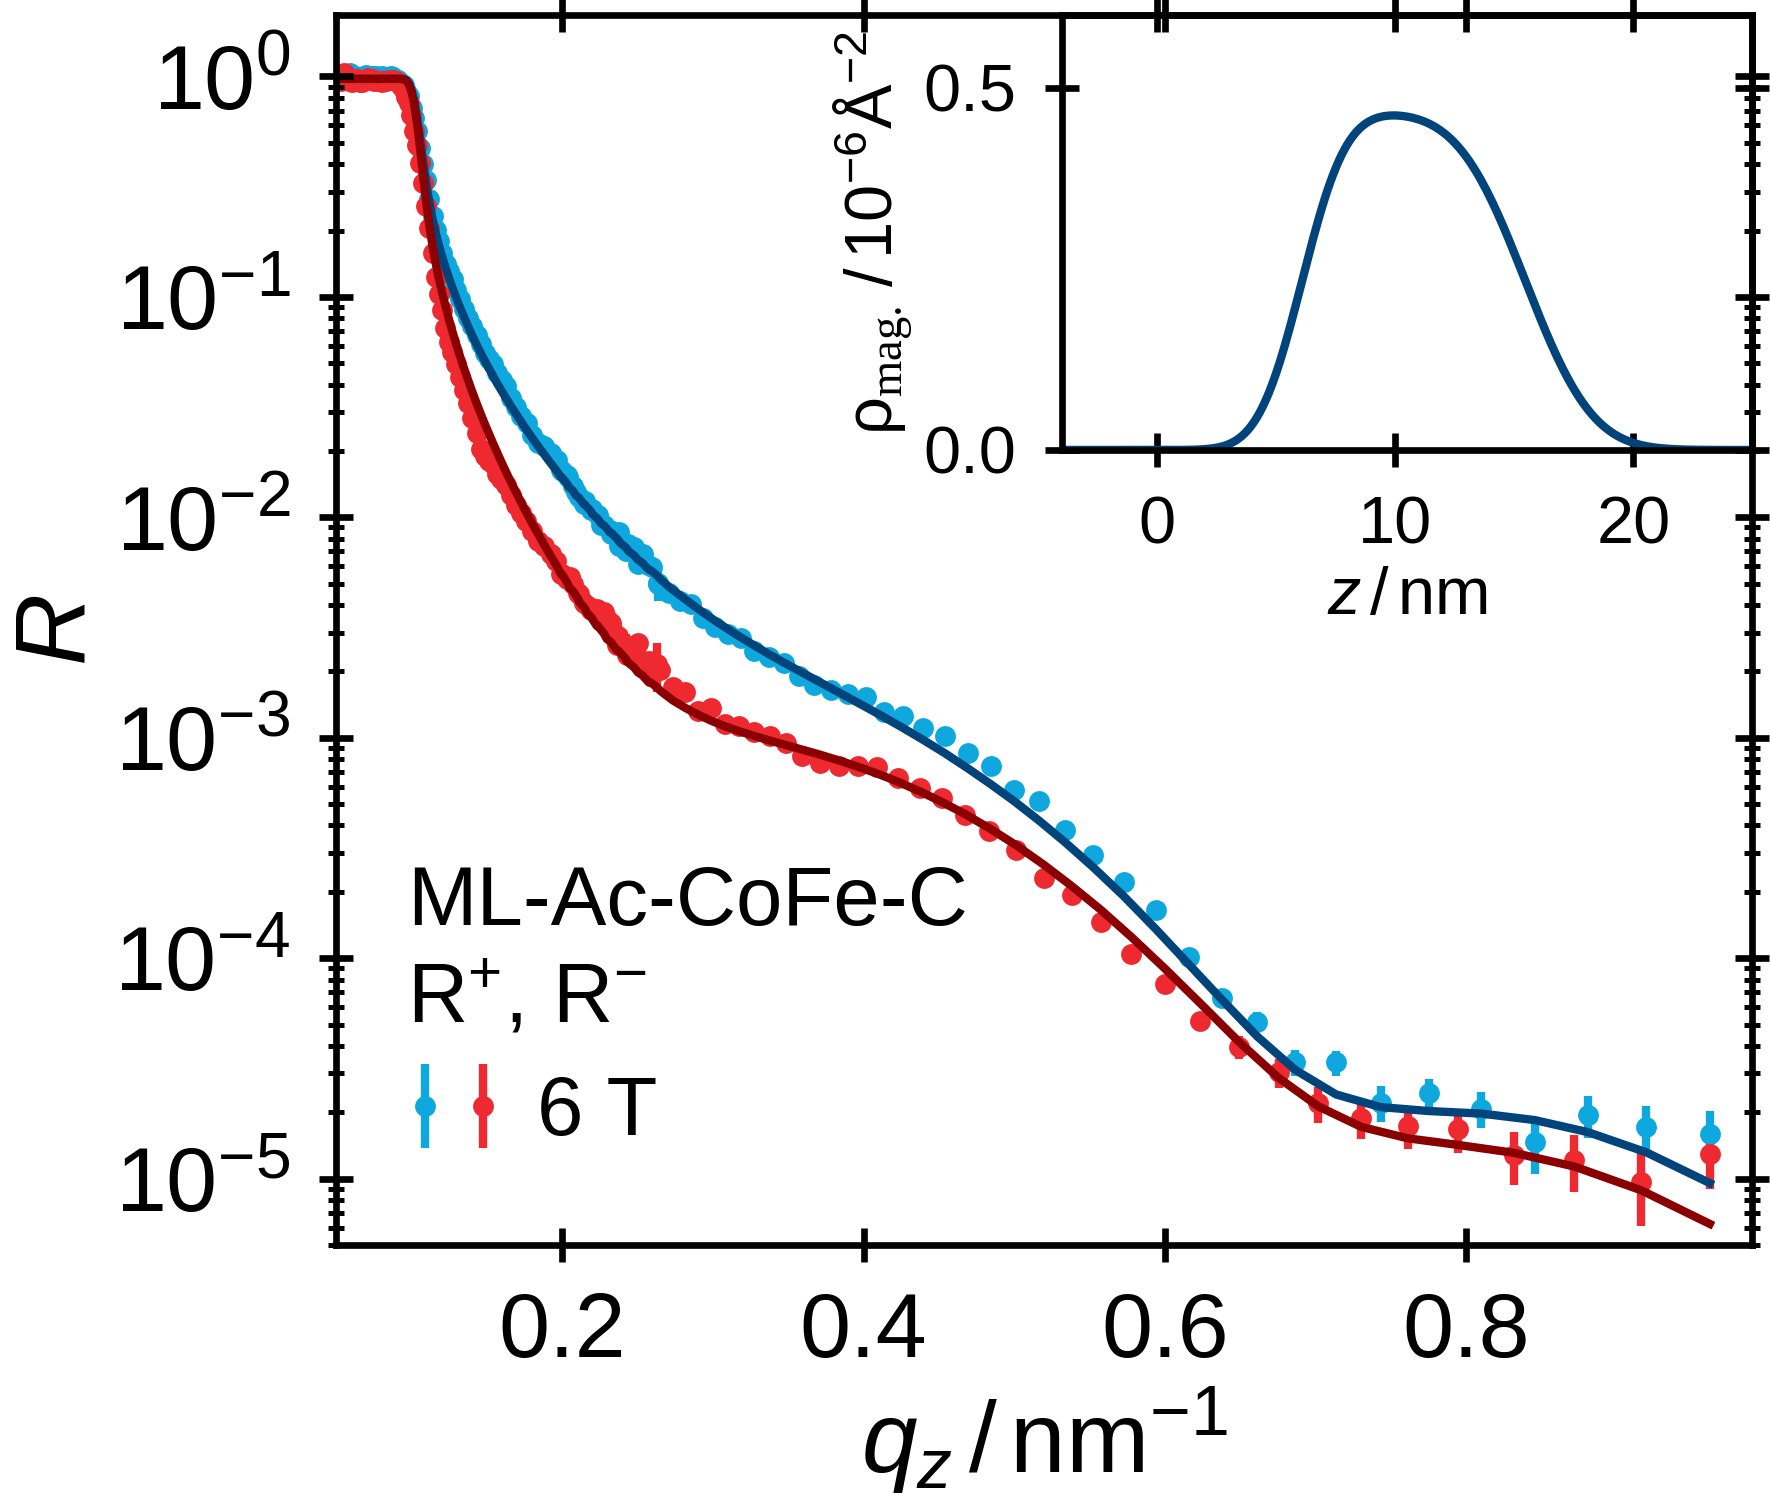
\includegraphics{monolayers_MagneticStructure_Ac-CoFe-C_PNR_ZFC5K_6T}
    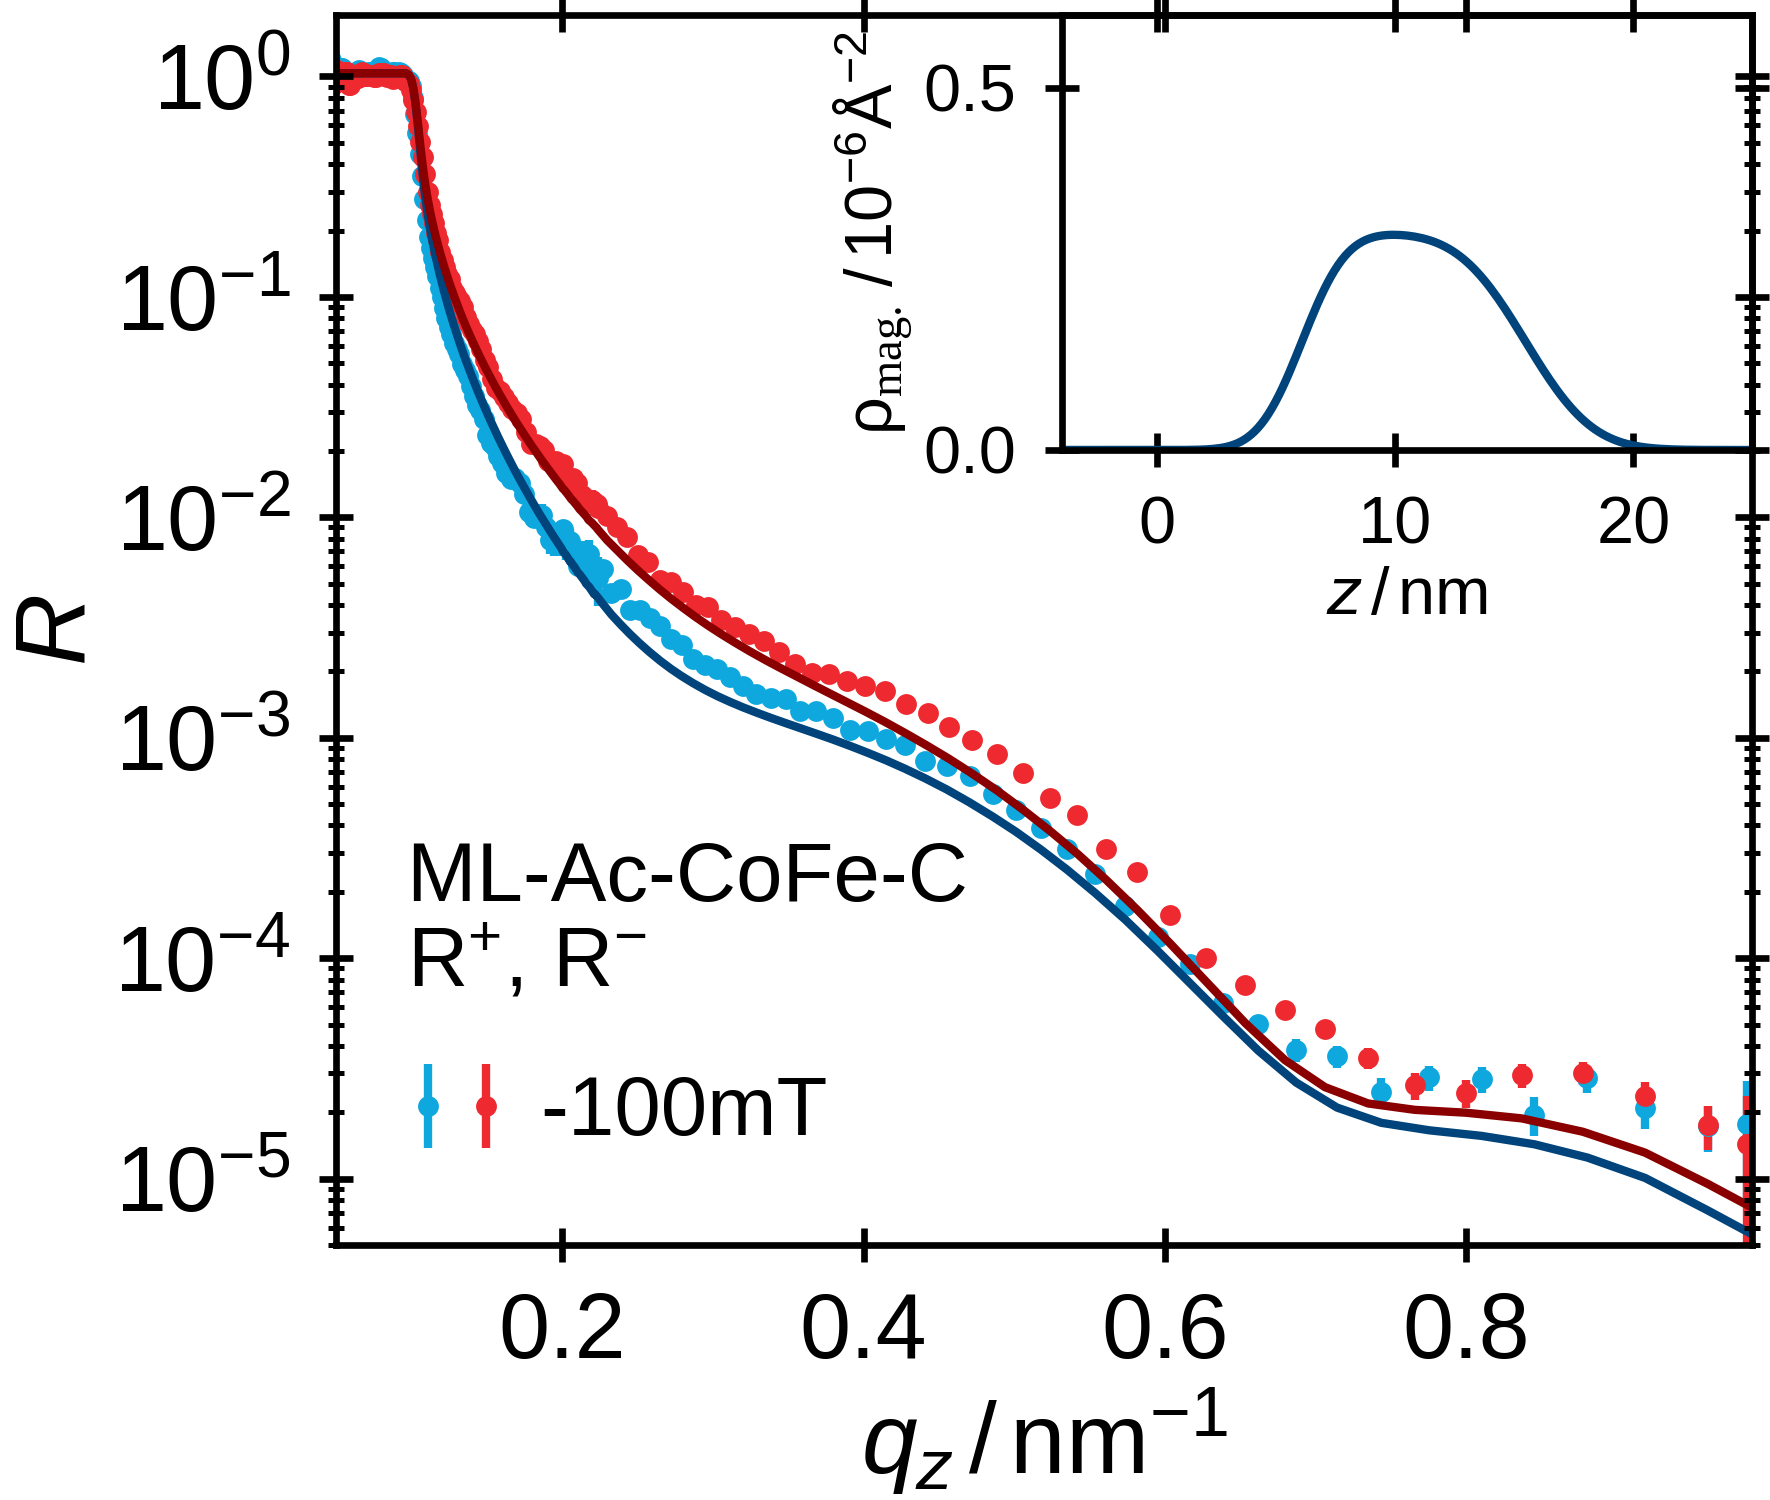
\includegraphics{monolayers_MagneticStructure_Ac-CoFe-C_PNR_ZFC5K_neg100mT}
    \caption{\label{fig:monolayer:magneticStructure:pnr5K}Polarized neutron reflectivity of Ac-CoFe-C-2 after zero-field cooling to $5 \unit{K}$ measured first at a magnetic field of $6 \unit{T}$ (left) and then at $-100 \unit{mT}$ (right). $R^{+}$ and $R^{-}$ correspond to the states of the RF flipper turned off and on respectively. The calculated reflectivities are obtained from using the nuclear structure determined in \refsec{sec:monolayers:structure:verticalModel}, and the magnetic SLD shown in the inset.}
  \end{figure}
  The reflectivities under an applied in-plane magnetic field $\vec{B}_\mathrm{ext.}$ of ML-Ac-CoFe-C for incident neutrons with the the RF flipper turned off $R^{+}$ and with the flipper turned on $R^{-}$ are shown in \reffig{fig:monolayer:magneticStructure:pnr5K}.
  A splitting between both channels is clearly visible at both a large field of $6 \unit{T}$, as well subsequently at $-100 \unit{mT}$.
  At the saturating field of $6 \unit{T}$ it is visible that $R^{+} > R^{-}$, which corresponds to a homogeneous sample magnetization parallel to the applied field as expected.
  At the negative field the two curves flip and $R^{-} > R^{+}$, which can be connected to the switched role of the two states with respect to the external magnetic field direction.
  Thus the flipping of the two states corresponds still to the same magnetization direction as in the saturated state, as is expected from the macroscopic vibrating sample magnetization measurement at $5 \unit{K}$ in \reffig{fig:monolayer:magneticStructure:MLAcCoFeC}.

  With the nuclear scattering length density profile determined in \refsec{sec:monolayers:structure:verticalModel}, the magnetization scattering length density of the nanocubes in the monolayer can be quantitatively discussed.
  Using the same parameterized scattering length density profile for $\rho_\mathrm{mag.}$ as is used for $\rho_\mathrm{nuc.}$, with every material but the nanocube having zero magnetic SLD, the reflectivities are refined by the single parameter describing nanocube magnetization $\rho_\mathrm{mag.}^\mathrm{NC}$.
  The best fit values are tabulated in \reftab{tab:monolayers:magneticStructure:pnrResult}.
  For the $6 \unit{T}$ measurement, a value of $316(7) \unit{kA \, m^{-1}}$ is obtained and at $-100 \unit{T}$ the best fit corresponds to $206(14) \unit{kA \, m^{-1}}$.

  \begin{table}[!htbp]
    \centering
    \caption{\label{tab:monolayers:magneticStructure:pnrResult}Magnetic scattering length density $\rho_\mathrm{mag.}^\mathrm{NC}$ of the nanocube layer determined from PNR shown in \reffig{fig:monolayer:magneticStructure:pnr5K}. The fitted value is transformed to a volume magnetization $M$ by \refeq{eq:theoreticalBackground:scattering:magneticSLD}.}
    \begin{tabular}{l | c | c}
      \hline
      PNR & \textbf{6 T} & \textbf{-100 mT}\\
      \hline
      $\rho_\mathrm{mag.}^\mathrm{NC}\, / \unit{10^{-6} \angstrom^{-2}}$ & $0.92(2)$  & $0.60(4)$  \\
      \hline
      $M \, / \unit{kA \, m^{-1}}$                                       & $316(7)$   & $206(14)$  \\
      \hline
      \end{tabular}
  \end{table}

  The saturated state at $6 \unit{T}$ is well described by the homogeneous magnetization for the whole measured range in \reffig{fig:monolayer:magneticStructure:pnr5K}.
  The state measured at a negative field afterwards shows however slight deviations.
  At low scattering vectors $q < 0.2 \unit{\angstrom^{-1}}$, the splitting is still well described by the used model, but at the higher range, the experimental data is for both channels more intense than would be expected.
  This can also not be corrected by reducing the size of the nanocube layer in the magnetic scattering density profile, which can be done by introducing more parameters.

  The obtained magnetizations can be compared to the magnitude of magnetization observed with VSM at $5 \unit{K}$, where a magnetization of $358(13) \unit{kA \, m^{-1}}$ is obtained at $6 \unit{T}$ and $247(2) \unit{kA \, m^{-1}}$ at $-100 \unit{mT}$.
  The relative reduction of the magnetization to $65 \%$ of the saturated magnetization from $6 \unit{T}$ to $-100 \unit{mT}$ is in agreement by both experiments.
  In absolute units, VSM resulted in approximately $15 \%$ larger values in both cases.
  As the VSM does not provide the magnetization scaled to the volume, but has to be rescaled by an estimate of the magnetic sample volume, this deviation corresponds to the systematic error.
  In this case it was chosen to scale to the magnetization estimated from the nanocube magnetic moment in dispersion and size determined from SAS.
  Using PNR it is shown that this approach overestimates the sample magnetization slightly and a reduced value is actually observed in the ordered monolayer sample.


\end{document}